%%%%%%%%%%%%%%%%%%%%%%%%%%%%%%%%%%%%%%%%%
% a0poster Portrait Poster
% LaTeX Template
% Version 1.0 (22/06/13)
%
% The a0poster class was created by:
% Gerlinde Kettl and Matthias Weiser (tex@kettl.de)
% 
% This template has been downloaded from:
% http://www.LaTeXTemplates.com
%
% License:
% CC BY-NC-SA 3.0 (http://creativecommons.org/licenses/by-nc-sa/3.0/)
%
%%%%%%%%%%%%%%%%%%%%%%%%%%%%%%%%%%%%%%%%%

%----------------------------------------------------------------------------------------
%	PACKAGES AND OTHER DOCUMENT CONFIGURATIONS
%----------------------------------------------------------------------------------------

\documentclass[portrait,a1]{a0poster}

\usepackage{multicol} % This is so we can have multiple columns of text side-by-side
\columnsep=100pt % This is the amount of white space between the columns in the poster
\columnseprule=3pt % This is the thickness of the black line between the columns in the poster

\usepackage[svgnames]{xcolor} % Specify colors by their 'svgnames', for a full list of all colors available see here: http://www.latextemplates.com/svgnames-colors

%x\usepackage{times} % Use the times font
\usepackage{palatino} % Uncomment to use the Palatino font

\usepackage{graphicx} % Required for including images
\graphicspath{{figures/}} % Location of the graphics files
\usepackage{booktabs} % Top and bottom rules for table
\usepackage[font=small,labelfont=bf]{caption} % Required for specifying captions to tables and figures
\usepackage{amsfonts, amsmath, amsthm, amssymb} % For math fonts, symbols and environments
\usepackage{wrapfig} % Allows wrapping text around tables and figures
%\usepackage{subfig}
\usepackage{float}
\usepackage[it]{subfigure}
\usepackage{epstopdf}

\begin{document}

%----------------------------------------------------------------------------------------
%	POSTER HEADER 
%----------------------------------------------------------------------------------------

% The header is divided into two boxes:
% The first is 75% wide and houses the title, subtitle, names, university/organization and contact information
% The second is 25% wide and houses a logo for your university/organization or a photo of you
% The widths of these boxes can be easily edited to accommodate your content as you see fit



\begin{minipage}[b]{0.85\linewidth}
\Huge \color{NavyBlue} \textbf{Hierarchical Controller Architecture} \color{Black}\\[0.5cm] % Title
\Huge\color{NavyBlue}\text{in Software Defined Networks}\\[1cm] % Subtitle
\Large \text{Gourav Khaneja, Sweta Seethamraju \& Praveen Kumar}\\[0.5cm] % Author(s)

%\huge University and Department Name\\[0.4cm] % University/organization
%\Large \texttt{john@LaTeXTemplates.com} --- 1 (000) 111 1111\\
\end{minipage}
%
\begin{minipage}[b]{0.15\linewidth}

\includegraphics[scale=0.8]{UIUC_logo.png}\\
\end{minipage}


\vspace{-1cm} % A bit of extra whitespace between the header and poster content

%----------------------------------------------------------------------------------------

\begin{multicols}{2} % This is how many columns your poster will be broken into, a portrait poster is generally split into 2 columns

%----------------------------------------------------------------------------------------
%	ABSTRACT
%----------------------------------------------------------------------------------------

%\color{Navy} % Navy color for the abstract
%
%\begin{abstract}
%
%Sed fringilla tempus hendrerit. Vestibulum ante ipsum primis in faucibus orci luctus et ultrices posuere cubilia Curae; Etiam ut elit sit amet metus lobortis consequat sit amet in libero. Lorem ipsum dolor sit amet, consectetur adipiscing elit. Phasellus vel sem magna. Nunc at convallis urna. isus ante. Pellentesque condimentum dui. Etiam sagittis purus non tellus tempor volutpat. Donec et dui non massa tristique adipiscing. Quisque vestibulum eros eu. Phasellus imperdiet, tortor vitae congue bibendum, felis enim sagittis lorem, et volutpat ante orci sagittis mi. Morbi rutrum laoreet semper. Morbi accumsan enim nec tortor consectetur non commodo nisi sollicitudin. Proin sollicitudin. Pellentesque eget orci eros. Fusce ultricies, tellus et pellentesque fringilla, ante massa luctus libero, quis tristique purus urna nec nibh.
%
%\end{abstract}

%----------------------------------------------------------------------------------------
%	INTRODUCTION
%----------------------------------------------------------------------------------------

%\color{SaddleBrown} % SaddleBrown color for the introduction
%
%\section*{Introduction}
%
%Aliquam non lacus dolor, \textit{a aliquam quam} \cite{Smith:2012qr}. Cum sociis natoque penatibus et magnis dis parturient montes, nascetur ridiculus mus. Nulla in nibh mauris. Donec vel ligula nisi, a lacinia arcu. Sed mi dui, malesuada vel consectetur et, egestas porta nisi. Sed eleifend pharetra dolor, et dapibus est vulputate eu. \textbf{Integer faucibus elementum felis vitae fringilla.} In hac habitasse platea dictumst. Duis tristique rutrum nisl, nec vulputate elit porta ut. Donec sodales sollicitudin turpis sed convallis. Etiam mauris ligula, blandit adipiscing condimentum eu, dapibus pellentesque risus.
%
%\textit{Aliquam auctor}, metus id ultrices porta, risus enim cursus sapien, quis iaculis sapien tortor sed odio. Mauris ante orci, euismod vitae tincidunt eu, porta ut neque. Aenean sapien est, viverra vel lacinia nec, venenatis eu nulla. Maecenas ut nunc nibh, et tempus libero. Aenean vitae risus ante. Pellentesque condimentum dui. Etiam sagittis purus non tellus tempor volutpat. Donec et dui non massa tristique adipiscing.
%
%----------------------------------------------------------------------------------------
%	OBJECTIVES
%----------------------------------------------------------------------------------------

\color{SaddleBrown}% DarkSlateGray color for the rest of the content
\section*{PROBLEM}
\color{DarkSlateGray}
\begin{tabular} {l | l}
    \textbf{Single Controller Architecture} & \textbf{Distributed controller Architecture} \\
    \hline
    Responsiveness & Communication overhead \\
       Scalability & Scalability of global network view \\
       Reliability & Network state inconsistencies \\
                   & Management barriers across networks
\end{tabular}

\textbf{Trade-offs}
\begin{itemize}
    \item Consistency vs. Responsiveness
    \item Optimality vs. I dont know what
    \item Application design complexity (Architecture aware vs. agnostic)\\
\end{itemize}

\textbf{Goals}
\begin{itemize}
    \item Make control applications agnostic to architecture
    \item Reduce communication overhead
    \item Minimize network state inconsistencies
    \item Enable smooth transition across management barriers
    \item Handle changes locally \\
\end{itemize}

\textbf{Price we pay}
\begin{itemize}
    \item Solution not always optimal
\end{itemize}

\color{SaddleBrown}
\section*{PROPOSED SOLUTION}
\color{DarkSlateGray}
\begin{itemize}
    \item Hierarchical arrangement of controllers
    \item One switch abstraction
    \item Translate messages across hierarchical layers
\end{itemize}

\begin{figure}[H]
\centering
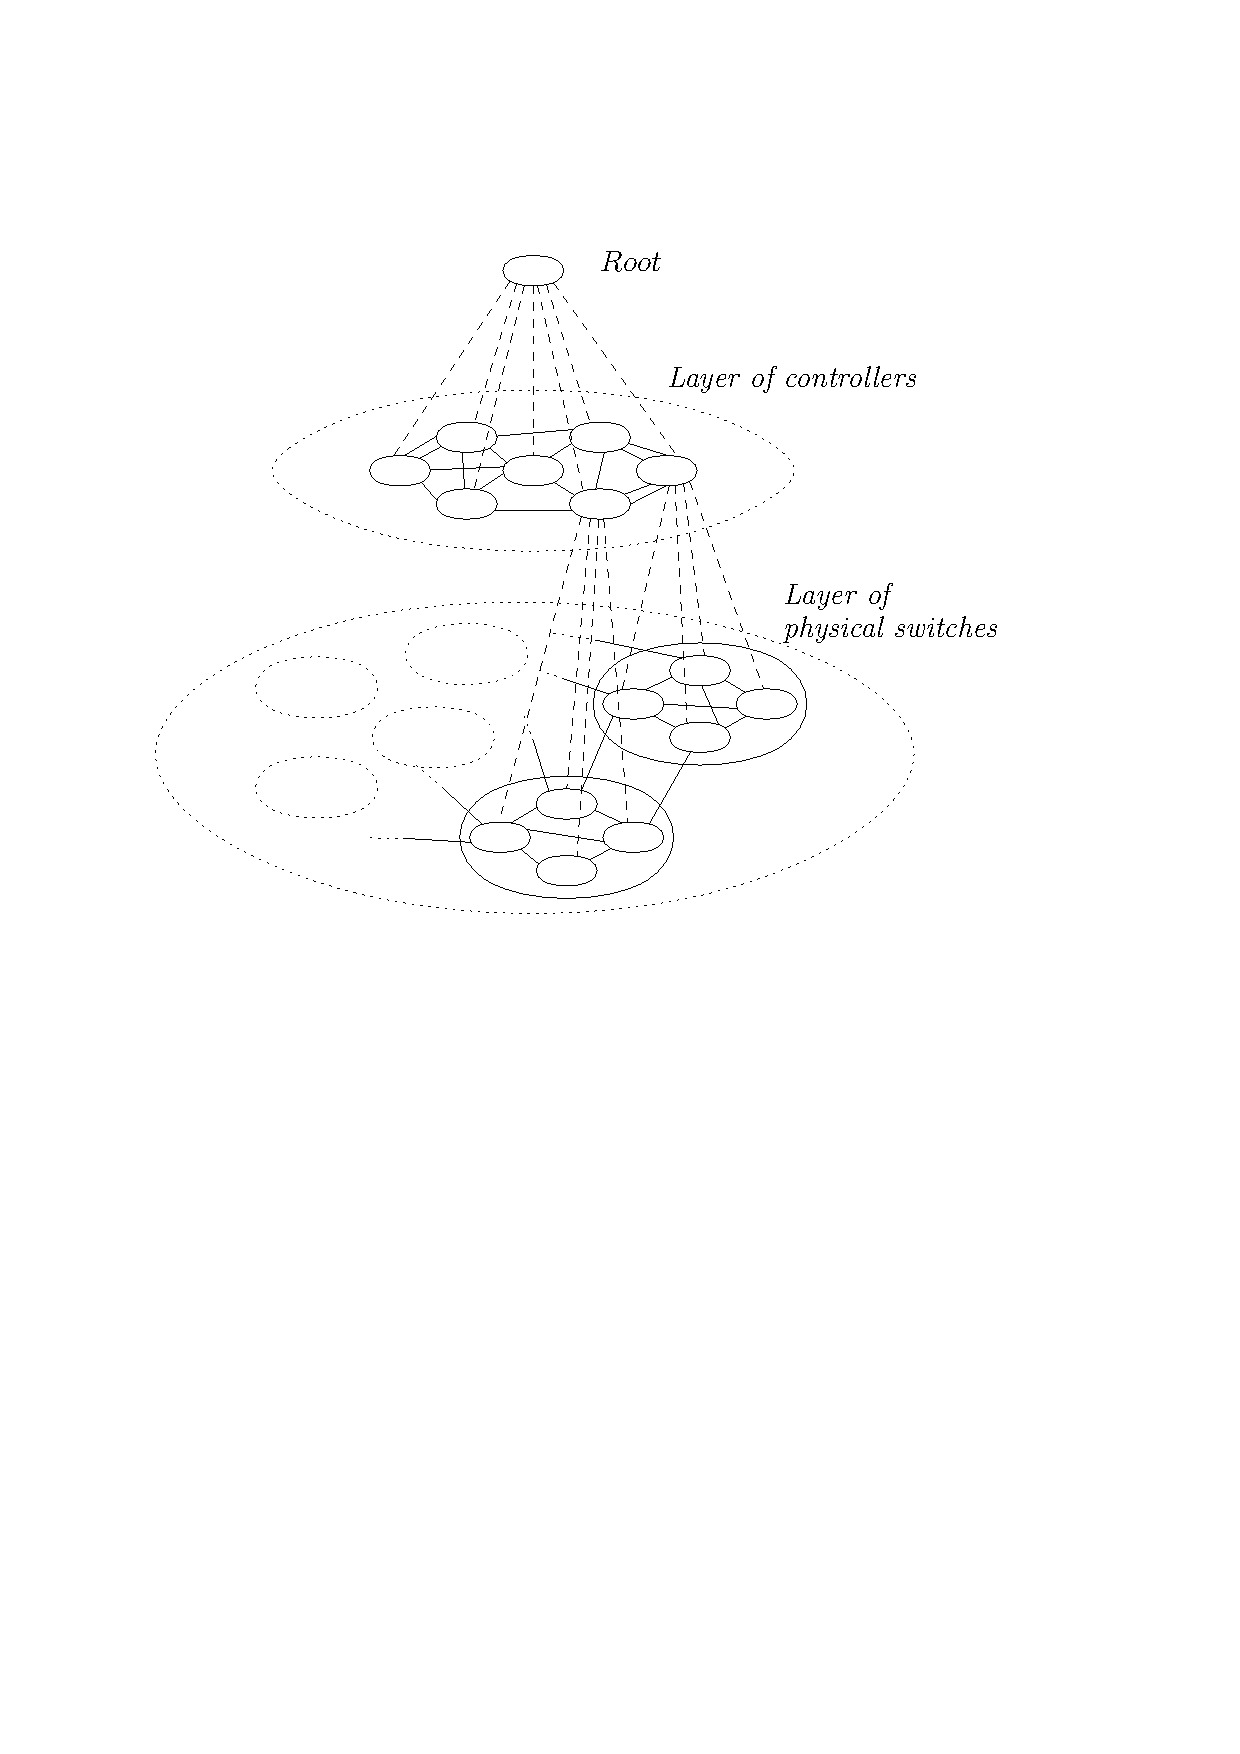
\includegraphics[scale=1.9]{hierarchy}
\caption{Hierarchical arrangement of controllers}
\label{fig:hierarchy}
\end{figure}


%------------------------------------------------




%Gourav - I'm starting from here ownwards: 
%----------------------------------------------------------------------------------------
%	RESULTS 
%----------------------------------------------------------------------------------------
\color{SaddleBrown}
\section*{EXPERIMENTAL SETUP}
\color{DarkSlateGray}
\begin{itemize}
%\item We simulated a dummy control application on both hierarchical and flat controller architectures, with same network topology and flow arrival distribution.
\item Flow data (6000 MapReduce jobs) was generated by sampling historical Hadoop traces on a 600 machine cluster at Facebook (1 million jobs). A dummy MapReduce application choses directory, map and reduce nodes randomly for each job.
\item Topology: 600 hosts connected through a network of 200 switches and 10 Gbps links. The cluster is divided into 10 equally-sized control domains.
\item TE-cum-routing coutrol application: When a new flow arrives, it finds the path with minimum maximum utilization. If multiple such paths exist (which is frequently the case, due to a large network), shortest path (in term of number of hops) is chosen.
\end{itemize}

\color{SaddleBrown}
\section*{METRICS}
\color{DarkSlateGray}
\begin{itemize}
\item Path length (number of hops) of the routes assigned to flows.
\item Maximum link utilization of the path assigned to flows.
\item Communication overhead (number of messages exchanged between controllers) for seting up routes for flows.   
\end{itemize}



%\begin{center}\vspace{1cm}
%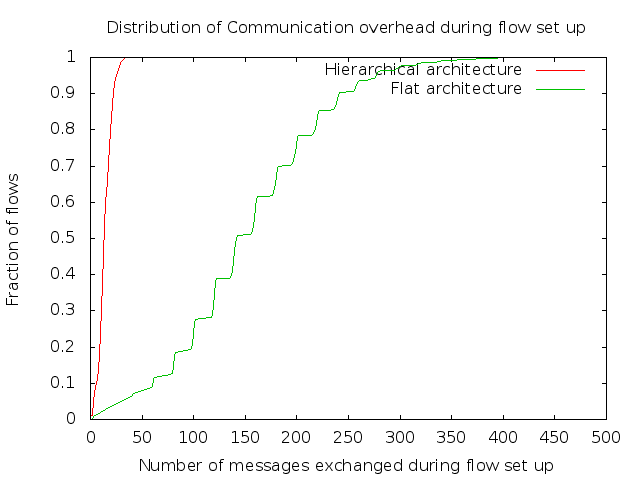
\includegraphics[width=0.8\linewidth]{msg}
%\captionof{figure}{\color{Green} Per flow communication overhead}
%\label{fig:msg}
%\end{center}\vspace{1cm}
\begin{figure}[H]
\centering
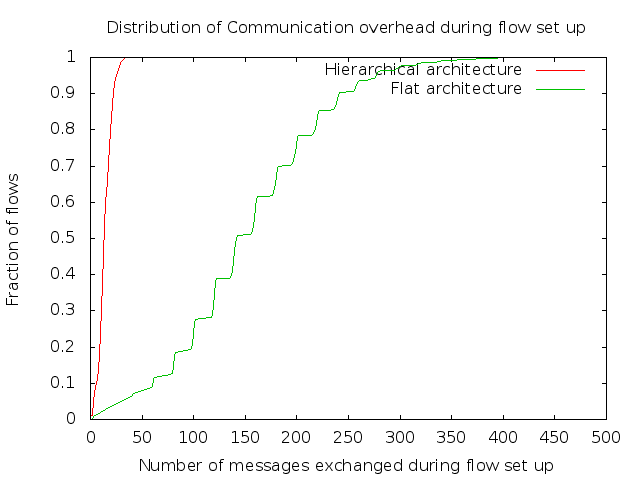
\includegraphics[scale=01]{msg}
\caption{Per flow communication overhead}
\label{fig:msg}
\end{figure}


%\begin{center}\vspace{1cm}
%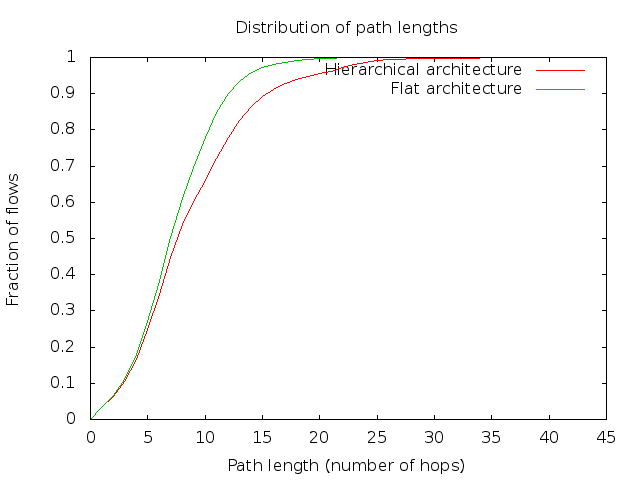
\includegraphics[width=0.5\linewidth]{path}
%\captionof{figure}{\color{Green} Path length (number of hops) assigned to flows}
%\end{center}\vspace{1cm}

%\begin{center}\vspace{1cm}
%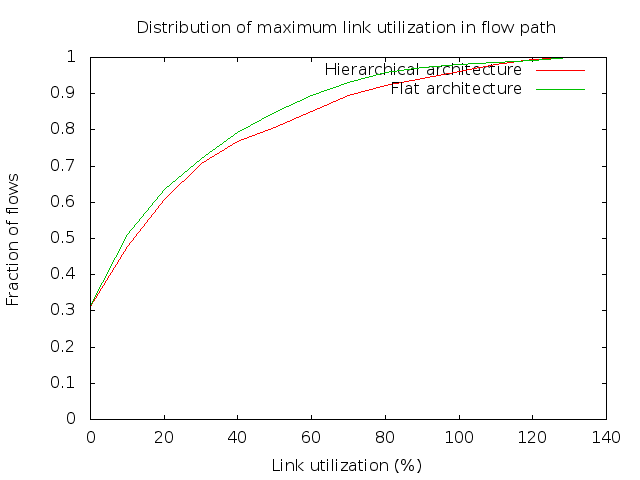
\includegraphics[width=0.5\linewidth]{util}
%\captionof{figure}{\color{Green} Maximum link utilization encountered by flows}
%\end{center}\vspace{1cm}

\begin{figure}[H]
  \begin{center}  
    \subfigure[Path length]{\label{fig:path}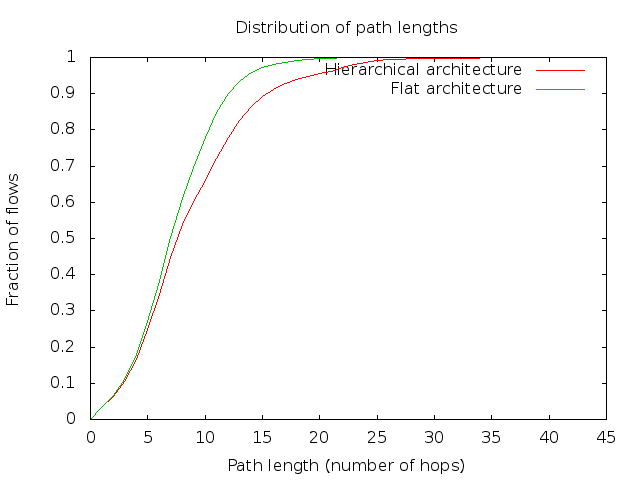
\includegraphics[scale=0.55]{path.png}} 
    \subfigure[Maximum link utilization]{\label{fig:util}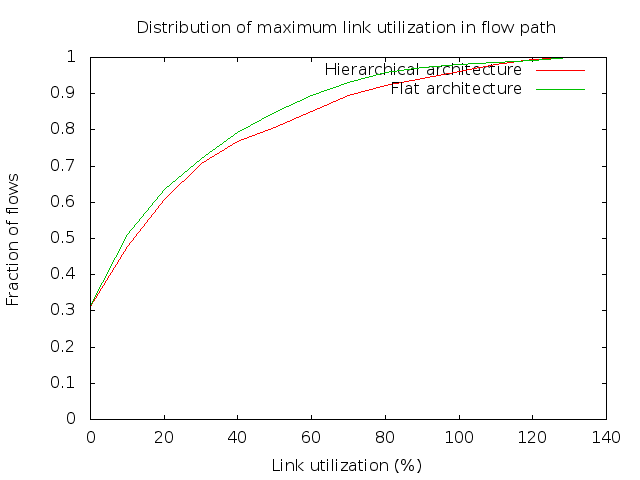
\includegraphics[scale=0.55]{util.png}} 
  \end{center}
\caption{Application performance}
\end{figure}

\color{SaddleBrown}
\section*{RESULTS}
\color{DarkSlateGray}
Hierarchical architecture reduces communication overhead (Figure \ref{fig:msg}) by an order of magnitude while comprimising modestly on optimality: shortest path length (17.4\%) (Figure \ref{fig:path}) and minimum maximum link utilization (12.8\%) (Figure \ref{fig:util}).

%----------------------------------------------------------------------------------------
%	CONCLUSIONS
%----------------------------------------------------------------------------------------

\color{SaddleBrown} % SaddleBrown color for the conclusions to make them stand out

%\section*{CONCLUSION}


\color{DarkSlateGray} % Set the color back to DarkSlateGray for the rest of the content

%----------------------------------------------------------------------------------------
%	FORTHCOMING RESEARCH
%----------------------------------------------------------------------------------------

%\section*{Forthcoming Research}



 %----------------------------------------------------------------------------------------
%	REFERENCES
%----------------------------------------------------------------------------------------
\color{SaddleBrown}
\section*{RESOURCES}
\color{DarkSlateGray}
\section*{Source Code}
https://github.com/MugiwaraLuffy/ACN/
\nocite{*} % Print all references regardless of whether they were cited in the poster or not
%\bibliographystyle{plain} % Plain referencing style
\bibliography{sample} % Use the example bibliography file sample.bib

%----------------------------------------------------------------------------------------
%	ACKNOWLEDGEMENTS
%----------------------------------------------------------------------------------------



%----------------------------------------------------------------------------------------

\end{multicols}
\end{document}
